\section{Приложение ТЕСТ}
\verb|Задание.| Создать приложение для проведения тестирования. \newline Должно содержать:
\begin{enumerate}
    \item Набор вопросов по какой-то теме (и вопросы и ответы должны быть реальные) "--- не менее 10
    \item Вопросы должны выбираться случайным образом.
    \item Вопросы должны быть нескольких типов "--- "Да/нет", Выбор одного ответа, Выбор нескольких ответов, Короткий ответ.
    \item Необходимо создать сообщения для правильного и неправильного ответа (Молодец, Не правильно и т.д.)
    \item Необходимо подсчитать количество правильных ответов и вывести результат.
\end{enumerate}

Для выполнения данного задания была разработана форма, содержащая два элемента 
\verb|TextBox|, четыре элемента \verb|GroupBox|, шесть элементов \verb|RadioButton|, 
четыре элемента \verb|CheckBox| и один элемент \verb|Button| (см. рисунок \ref{fig:test_const}).
\begin{figure}[H]
\centering
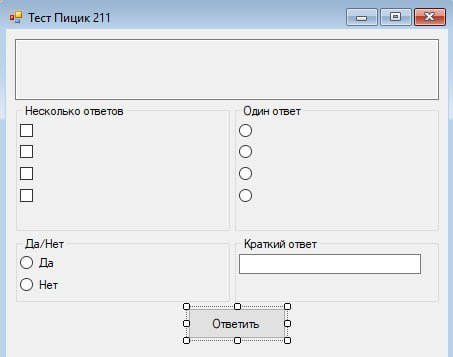
\includegraphics[scale=.85]{../img/test/test_const.jpg}
\caption{Окно приложения <<Тест>> открытое в конструкторе}
\label{fig:test_const}
\end{figure}

У элементов формы изменены значения некоторых свойств. Значения изменённых атрибутов 
представлены в таблицах \ref{tab:test} и \ref{tab:test_1}.
\begin{table}[H]
    \small
    \caption{Значение артибутов элементов формы, часть 1}
    \begin{tabular}{|l|l|}\hline
        \multicolumn{2}{|l|}{Форма}\cr\hline
        \verb"Text" & Тест Пицик 211 \cr\hline
        \multicolumn{2}{|l|}{Окно вывода вопросов}\cr\hline
        \verb"(Name)" & text\_questions \cr\hline
        \verb"ReadOnly" & True \cr\hline
        \multicolumn{2}{|l|}{Группа для нескольких ответов}\cr\hline
        \verb"(Name)" & group\_multiple \cr\hline
        \verb"Text" & Несколько ответов \cr\hline
        \multicolumn{2}{|l|}{Несколько ответов: 1"=й вариант}\cr\hline
        \verb"(Name)" & check\_1 \cr\hline
        \verb"Text" & \cr\hline
        \multicolumn{2}{|l|}{Несколько ответов: 2"=й вариант}\cr\hline
        \verb"(Name)" & check\_2 \cr\hline
        \verb"Text" & \cr\hline
        \multicolumn{2}{|l|}{Несколько ответов: 3"=й вариант}\cr\hline
        \verb"(Name)" & check\_3 \cr\hline
        \verb"Text" & \cr\hline
        \multicolumn{2}{|l|}{Несколько ответов: 4"=й вариант}\cr\hline
        \verb"(Name)" & check\_4 \cr\hline
        \verb"Text" & \cr\hline
        \multicolumn{2}{|l|}{Группа для одного ответа}\cr\hline
        \verb"(Name)" & group\_single \cr\hline
        \verb"Text" & Один ответ \cr\hline
        \multicolumn{2}{|l|}{Один ответ: 1"=й вариант}\cr\hline
        \verb"(Name)" & radio\_single1 \cr\hline
        \verb"Text" & \cr\hline
        \multicolumn{2}{|l|}{Один ответ: 2"=й вариант}\cr\hline
        \verb"(Name)" & radio\_single2 \cr\hline
        \verb"Text" & \cr\hline
        \multicolumn{2}{|l|}{Один ответ: 3"=й вариант}\cr\hline
        \verb"(Name)" & radio\_single3 \cr\hline
        \verb"Text" & \cr\hline
        \multicolumn{2}{|l|}{Один ответ: 4"=й вариант}\cr\hline
        \verb"(Name)" & radio\_single4 \cr\hline
        \verb"Text" & \cr\hline
    \end{tabular}
    \label{tab:test}
\end{table}

\begin{table}[H]
\small
\caption{Значение артибутов элементов формы, часть 2}
\begin{tabular}{|l|l|}\hline
    \multicolumn{2}{|l|}{Группа для Да/Нет}\cr\hline
    \verb"(Name)" & group\_yesno \cr\hline
    \verb"Text" & Да/нет \cr\hline
    \multicolumn{2}{|l|}{Да/нет: да}\cr\hline
    \verb"(Name)" & radio\_yes \cr\hline
    \verb"Text" & Да \cr\hline
    \multicolumn{2}{|l|}{Да/нет: нет}\cr\hline
    \verb"(Name)" & radio\_no \cr\hline
    \verb"Text" & Нет \cr\hline
    \multicolumn{2}{|l|}{Группа для краткого ответа}\cr\hline
    \verb"(Name)" & group\_txt \cr\hline
    \verb"Text" & Краткий ответ \cr\hline
    \multicolumn{2}{|l|}{Краткий ответ: текст}\cr\hline
    \verb"(Name)" & text\_answer \cr\hline
    \multicolumn{2}{|l|}{Кнопка для ответа}\cr\hline
    \verb"(Name)" & btn\_answer \cr\hline
    \verb"Text" & Ответить \cr\hline
\end{tabular}
\label{tab:test_1}
\end{table}

Были созданы отдельные структуры для отслеживания типа вопроса, \newline вариантов ответа и правильного ответа:
\begin{minted}[linenos, breaklines=true, style=bw, fontsize=\small]{cpp}
// структура для Теста
public enum struct Test
    {
        yes_no,
        single,
        multiple,
        txt_answer
    };

    //структура вопросов
    public ref struct Questions
    {
        System::String^ text; //формулировка вопроса
        array<System::String^>^ answers; //варианты ответа
        Test type; //тип ответа
        System::Object^ answer; //ответ 
    };
\end{minted}

Была создана отдельная функция для перемешивания всех вопросов:
\begin{minted}[linenos, breaklines=true, fontsize=\small, style=bw]{cpp}
// функция для перемешивания вопросов
void randomize_questions(array<Questions^>^ arr) {
        Random^ rand = gcnew Random();
        for (int i = arr->Length - 1; i > 0; --i)
        {
            int j = rand->Next(0, i + 1);

            Questions^ temp = arr[i];
            arr[i] = arr[j];
            arr[j] = temp;
        }
    }
\end{minted}

Фрагмент массива, содержащего все вопросы для теста:
\begin{minted}[linenos, style=bw, fontsize=\small, breaklines=true]{cpp}
//массив всех вопросов 
array<Questions^>^ test_dataset() {
    array<Questions^>^ q = gcnew array<Questions^>(12);

    q[0] = gcnew Questions();
    q[0]->text = "C++, Python, C - это всё ______ (полное словосочетание)";
    q[0]->type = Test::txt_answer;
    q[0]->answer = "языки программирования";

    q[1] = gcnew Questions();
    q[1]->text = "Какой тип данных описывает целочисленный тип?";
    q[1]->type = Test::single;
    q[1]->answers = gcnew array<String^>{ "integer", "float", "boolean", "string" };
    q[1]->answer = 0;
\end{minted}

С остальными кодами можно ознакомиться в приложении \ref{app:codes}.

После запуска приложения появляется окно (см. рисунок \ref{fig:test_res}).
\begin{figure}[H]
    \centering
    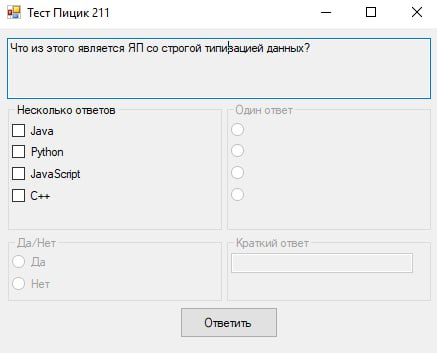
\includegraphics[scale=.85]{../img/test/test_res.jpg}
    \caption{Окно приложения <<Тест>>: начальный запуск}
    \label{fig:test_res}
\end{figure}

При выборе правильного варианта ответа появляется \verb|MessageBox| с надписью
(см. рисунок \ref{fig:test_correct}).
\begin{figure}[H]
\centering
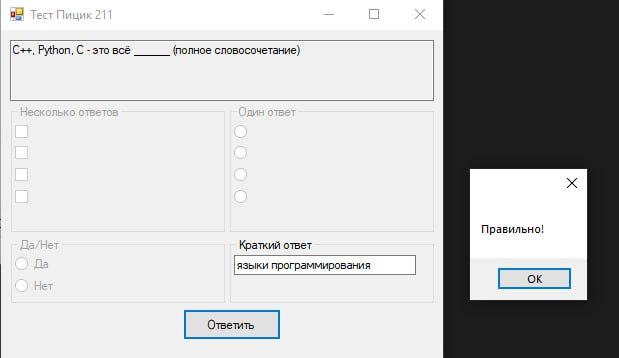
\includegraphics[scale=.85]{../img/test/test_correct.jpg}
\caption{<<Тест>>: выбор правильного ответа}
\label{fig:test_correct}
\end{figure}

При выборе неправильного варианта, выводится другое сообщение (см. рисунок \ref{fig:test_incorrect}).
\begin{figure}[H]
    \centering
    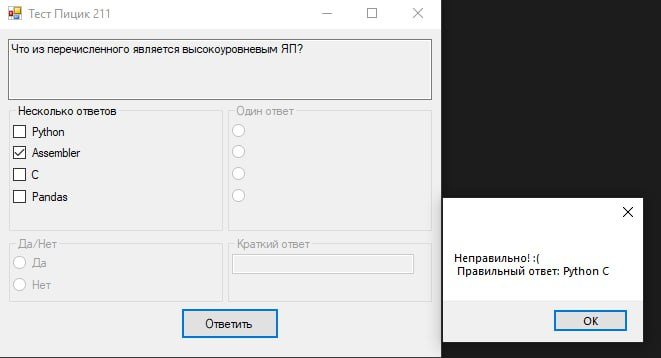
\includegraphics[scale=.85]{../img/test/test_incorrect.jpg}
    \caption{<<Тест>>: выбор неправильного ответа}
    \label{fig:test_incorrect}
\end{figure}

По прохождению теста выводится сообщение о завершении теста, а также счёт пользователя (см. рисунок \ref{fig:test_finish}).
\begin{figure}[H]
    \centering
    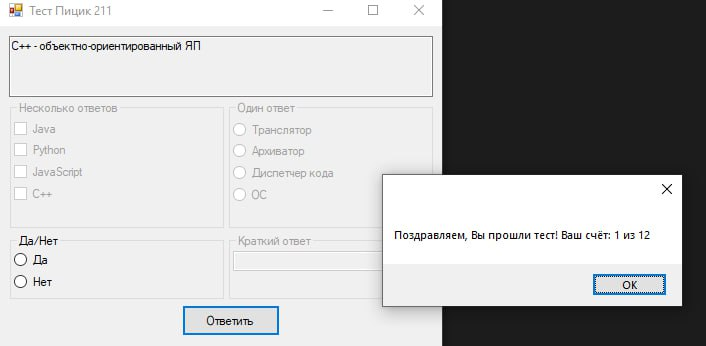
\includegraphics[scale=.85]{../img/test/test_finish.jpg}
    \caption{<<Тест>>: завершение теста}
    \label{fig:test_finish}
\end{figure}

С полным кодом программы можно ознакомиться в приложении \ref{app:repo}.